\begin{frame}{Question 1}
\begin{block}{Question}
What is the relation between the results presented in the Table 1 of the paper on the Neural Precedence Recommender and the size of the set of created search space nodes during the created proofs?
\end{block}
\only<1>{\includegraphics[page=14,viewport=80 350 380 430,clip]{papers/2021-cade}}
%\includepdf[pages=14,viewport=80 350 380 430,scale=\textbf{}.1,clip,frame]{papers/2021-cade}
\only<2>{\begin{exampleblock}{Answer}
\centering
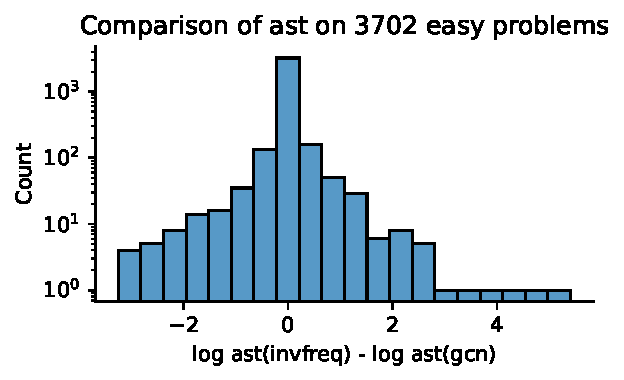
\includegraphics[scale=.5]{data/ast.pdf}
\end{exampleblock}}
\end{frame}
\begin{frame}{Question 2}
\begin{block}{Question}
What methods are considered to be applied for integration of the proving strategy and schedule optimization?
\end{block}
\begin{exampleblock}{Answer}
Combine \gls{smbo} with fast schedule optimization. Iteratively construct a portfolio:
\begin{enumerate}
\item Train a probabilistic \gls{epm}.
\item Estimate value of new strategies using the \gls{epm},
empirical runtimes of the portfolio, and
fast schedule optimization.
\item Empirically evaluate the best strategy.
\item Expand the portfolio if the new strategy improves it.
\end{enumerate}
\end{exampleblock}
\end{frame}
\begin{frame}{Question 0}
\begin{block}{Question}
Will these datasets be available for re-use by public?
\end{block}
\begin{exampleblock}{Comment}
The source code has been published.

I hope to publish the datasets when I consolidate the results for my dissertation thesis.
\end{exampleblock}
\end{frame}
